%!TEX root = twig-language.tex

\section{Code generation}
\label{sec:code-gen}

Twig is able to generate code in different target languages by
relying on an abstract, language-independent model with a small
number of basic operations. To implement a new target language, it
suffices to implement these operations only. In particular, there
is no need to modify the core Twig interpreter, which assumes only
the language-independent model.

We use the code generation model in describing Twig's semantics
(see Section~\ref{sec:semantics}). It is also helpful in
clarifying the precise operations which Twig supports, without
getting bogged down in the rather complicated details of rendering
code for a particular target language.

% TODO: maybe move the C section to Implementation? In
Section~\ref{sec:code-gen:abstract}, we describe the code
generation model abstractly, and apart from any specific target
language. Then, in Section~\ref{sec:code-gen:c}, we show how the
model can be specialized to generate C code.

\subsection{Abstract Code Generation}
\label{sec:code-gen:abstract}

We call a single unit of generated code a \emph{block}. A block is
an abstract representation of some code in a target language,
which accepts inputs and produces outputs. We denote the 
set of all blocks $M$, and provide functions 

\begin{eqnarray*}
\mbox{in} : M \to \mathbb{N}\\
\mbox{out} : M \to \mathbb{N}
\end{eqnarray*}

which map a block to the number of its inputs and outputs,
respectively.

\subsubsection{Sequential Composition}
\label{sec:code-gen:seq}

The first binary operation on blocks is \emph{sequential
composition}, which we represent as ``addition'' on the elements
of $M$, i.e.

\[
+ : M \times M \to M
\]

Sequencing represents connecting two blocks ``vertically,''
feeding the outputs of the first block to the inputs of the
second. The block $x+y \in M$ is defined if and only if
$\mbox{out}(x) = \mbox{in}(y)$. The outputs of the first element
must be equal in number to the inputs of the second element
because they are ``fused'' pairwise in the sequence operation. We
define

\[
\mbox{in}(x+y) = \mbox{in}(x)
\]

since the inputs of the first block will become the inputs of the
combined block. Similarly,

\[
\mbox{out}(x+y) = \mbox{out}(y)
\]

for the outputs.

\subsubsection{Parallel Composition}
\label{sec:code-gen:par}

The second block operator is \emph{parallel composition}. We
represent this operation as ``multiplication'' on the elements of
$M$, i.e.,

\[
\times : M \times M \to M
\]

Parallel composition attaches two blocks ``horizontally,'' where
each block executes independently of one another, but they appear
as a single block with combined inputs and outputs. For the block
$x\times y \in M$, we define

\[
\mbox{in} (x \times y) = \mbox{in}(x)+\mbox{in}(y)
\]

and

\[
\mbox{out}(x \times y) = \mbox{out}(x) + \mbox{out}(y)
\]

\subsubsection{Permutation and Identity Blocks}
\label{sec:code-gen:special}

We define a set of special blocks in $M$ called \emph{permutation}
blocks. These blocks represent the primitive operation of
``wiring'' $m$ inputs to $n$ outputs in arbitrary order, without
altering the values. Permutations may also ``drop'' an element by
not wiring its input to any output, and ``duplicate'' elements by
wiring an input to more than one output. The exact meaning of
dropping or duplicating values depends on the implementation.

We call the block permuting $m$ inputs to $n$ outputs\\
$\Pi_m(i_1,\ldots,i_n)$, where $i_1,\ldots,i_n \in \lbrace i \;|\;
1 \leq i \leq m \rbrace$.

\emph{Identity} blocks are a subset of the permutation blocks. The
simplest of these is $\Pi_1(1)$, which acts as an identity
transformation with one input and one output. That is, the block
$\Pi_1(1)$ takes its single input and passes it unchanged to its
single output. We refer to this block as $I_1$. There are an
unlimited number of identity transformations which take $n$ inputs
to $n$ outputs without reordering. We refer to these blocks as
$I_n$, where $1 \leq n$, and $I_n = \Pi_n(1,2,\ldots,n)$. By
definition, $\mbox{in}(I_n) = \mbox{out}(I_n) = n$.

When $n$ is implied from the context, we will sometimes write $I$
for $I_n$. For example, when we write $x+I$, we mean $x+I_n$ where
it is understood that $n = \mbox{out}(x)$.

Since the blocks $I$ represent identity operations, we assign them
a special meaning in the semantics. Namely, $I$ acts as both a
left- and right-identity under the sequence operator. So, for all
$x \in M$, $x + I = x$ and $I + x = x$. We usually use $I$ as a
``no-op'' block.

It is worth noting one further identity, namely that $I_n$ is
equivalent to the $n$-way parallel composition of $I_1$, that is

\[
I_n = \underbrace{I_1 \times \ldots \times I_1}_\text{n}
\]

Another important special block is the \emph{fanout} block, which
takes a single input and ``copies'' it to $n$ outputs. We denote
this block $F_n$. This turns out to be another special case of the
permutation block, and we can define

\[
F_n = \Pi_1(1,\ldots,n)
\]

to be the fanout block with $n$ outputs.

Note that \emph{any} object that provides and conforms to the
operations above can be ``generated'' by Twig. Because the system
is so general, this could include trivial or non-sensical
implementations. The code generation implementation should conform
to the intuitive interpretation of blocks and their composition.


\subsection{Generating C}
\label{sec:code-gen:c}

Now we show how we have adapted the model described above to
generate C code. Our implementation must provide a way to
construct a primitive block from an arbitrary chunk of C code
since the abstract model, by design, does not provide this
facility. In our implementation for C, a primitive block is a
string of C code with some specially-named variables indicating
inputs and outputs. In fact, our implementation makes no attempt
to parse the C language \emph{per se} -- it treats code as plain
text with the aforementioned special variables.

To use the block's inputs, the code references escaped variables
named \texttt{\$in1}, \texttt{\$in2}, and so on. Similarly, the
variables \texttt{\$out1}, \texttt{\$out2}, and so on represent
the outputs. We allow \texttt{\$in} as a synonym for
\texttt{\$in1}, and \texttt{\$out} for \texttt{\$out1}, for the
common case where a block has just one input and/or output. When
the code is rendered, these variables will be replaced with
unique, generated variable names. For example, the code

\begin{verbatim}
$out = foo($in);
\end{verbatim}

represents a primitive C block with one input and one output.
Figure~\ref{fig:blocks} shows a visual representation of two
primitive blocks of C code.

\begin{figure}[ht]
\centering
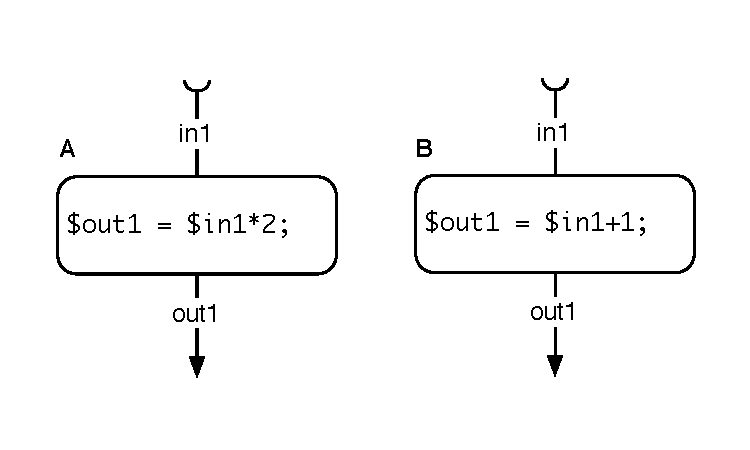
\includegraphics[width=0.75\columnwidth]{images/code-gen1}
\caption{Two basic blocks, $A$ and $B$. Inputs are on top, outputs 
on the bottom.}
\label{fig:blocks}
\end{figure}

To implement block sequencing in C, Twig generates variable names
such that the output(s) of the first block in the sequence are the
same as the inputs(s) of the second, and the text is concatenated.
See Figure~\ref{fig:codegen-seq} for an example.

\begin{figure}[ht]
\centering
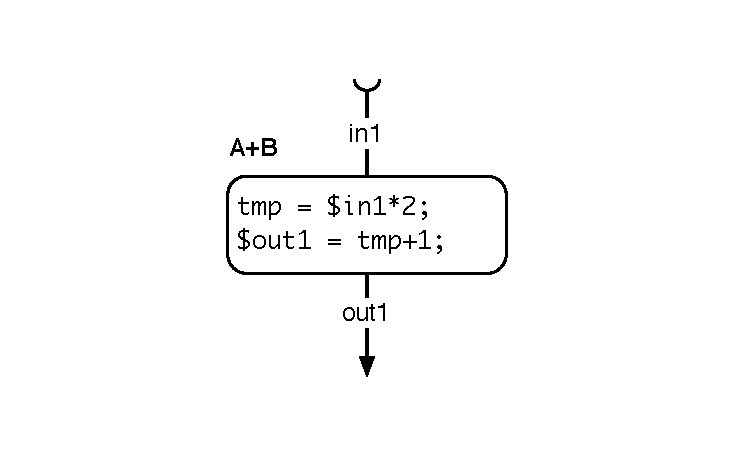
\includegraphics[width=0.75\columnwidth]{images/code-gen2}
\caption{Two blocks from Figure~\ref{fig:blocks} composed 
sequentially. The variable ``tmp'' is created, and renaming 
performed, so that the output of block $A$ would flow to the input 
of block $B$.}
\label{fig:codegen-seq}
\end{figure}

Parallel composition for C is implemented similarly; Twig
generates independently-named variables for the inputs and outputs
of the two blocks, and then concatenates the text. An example is
shown in Figure~\ref{fig:codegen-par}.

\begin{figure}[ht]
\centering
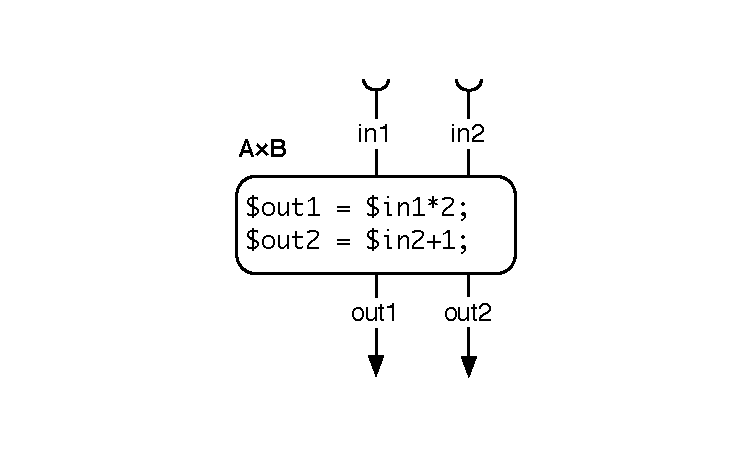
\includegraphics[width=0.75\columnwidth]{images/code-gen3}
\caption{Two blocks from Figure~\ref{fig:blocks} composed in 
parallel. Renaming is performed such that the composed block has 
two inputs and two outputs.}
\label{fig:codegen-par}
\end{figure}

Implementing the permutation and identity blocks is a matter of
performing the appropriate bookkeeping and renaming on the
variable names. Note that this implementation does not perform
resource management, such as allocating or free memory, as part of
the permutation operations. The generated code will follow C's
semantics for passing data by value.
